%==================================%
%-->    Lab: DC Voltage Divider <--%
%--> Author: Charles Edward Pax <--%
%-->   Date: Date lab began     <--%
%==================================%

% The README file contains much more detailed descriptions of all the commands you might need.

\documentclass[11pt,onecolumn]{article}
% This sets the document type to be used to "article" and activates any desired style optioins.
% Options
% ====================
% Name		Description
% --------	-----------
% 10pt		Set font size to 10 points
% 11pt		Set font size to 11 points
% 12pt		Set font size to 12 points
% onecolumn	Set number of columns to one
% twocolumn	Set number of columns to two

\usepackage{color}
\usepackage{graphics}
\usepackage{pstricks}
% Options
% ====================
% Name		Description
% --------	-----------
% color		Allows the inclusion of colors.
% graphics	Allows the inclusion of various graphics.
% pstricks	Allows many complex graphic functions such as circuit diagrams.

\begin{document}
% This command tells LaTeX to process the following commands as part of the document body.

\title{DC Voltage Divider}
% This command defines the title of the report for use in the "\maketitle" command below.

\date{\today}
% This command defines the date for use in the "\maketitle" command below. You may manually type any date or use one of the following options.
% Options
% ====================
% Name		Description
% --------	-----------
% \today	Includes the date the documents is compiled

\author{Charles Edward Pax}
% This command defines the author's name for use in the "\maketitle" command below.

\maketitle
% This command includes the title, author name, and date in the final document.

\abstract{Demonstrates the author's understanding of the DC voltage divider and basic electronic equipment, demonstrates the insuitability of a resistive voltage divider, and demonstrates the non-ohmic nature of a light-emitting diode.}
% This command tells LaTeX to format the contained text in a way particular to the abstract. The abstract is a breif paragraph describing the purpose, methods, and results of the experiment.

\section{Introduction}\label{sec:Introduction}
The resistive voltage divider in figure \ref{fig:Resistive_VD} is a simple device consisting of a voltage source and two resistors. The output voltage $V_{out}$ is related to $V_{in}$ by equation \ref{eq:V_out}. If $R_1 >> R_2$, $V_{out}$ varries almost linearly with $R_2$, while if $R_1 << R_2$, $V_{out}$, $V_{out} \approx V_{in}$.
\begin{figure}
\begin{center}
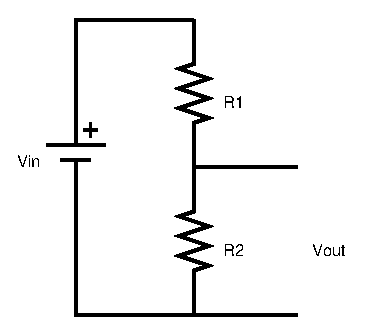
\includegraphics{Diagram1.eps}
\end{center}
%\input{Diagram1}
\caption{Resistive voltage divider.}\label{fig:Resistive_VD}
\end{figure}
\begin{equation}\label{eq:V_out}
V_{out} = V_{in} \frac{R_2}{R_1 + R_2}
\end{equation}

This is verified by working out the appropriate mathmatical expression shown in equation \ref{eq:Transform}\footnote{Answer to question one.}.
\begin{equation}\label{eq:Transform}
V_{out} = V_{in} \left(\left(\frac{R_2}{R_1}\right) - \left(\frac{R_2}{R_1}\right)^2\right)
\end{equation}

\section{Data \& Analysis}\label{sec:DataAnalysis}
\subsection{Part A}
A power supply provided the input voltage $V_{in} \approx 12$ V. Measurements for $V_{in}$ and $V_{out}$ were taken while setting $R_1$ = 100 k$\Omega$ for each value of $R_2$ = 1 $\Omega$, 10 $\Omega$, 100 $\Omega$, 1 k$\Omega$, 10 k$\Omega$, 100 k$\Omega$, 1 M$\Omega$. $R_1$ was reset to 100 $\Omega$ and the measurements for $V_{in}$ and $V_{out}$ repeated. Discrete components were used with their multimeter-measured values compared to their color-coded values in table \ref{fig:Resistors}.
\begin{table}
\begin{center}
\begin{tabular}{|r|r|}
\hline
Color Code ($\Omega$)	& Measured ($\Omega$) \\
\hline
1			& 1.1 \\
10			& 10.1 \\
100			& 99.7 \\
1000			& 985 \\
10000			& 9930 \\
100000			& 102600 \\
1000000			& 1069000 \\
\hline
\end{tabular}
\end{center}
\caption{Resistence in ohms given by the resistors' color codes and the measured resistences.}\label{fig:Resistors}
\end{table}

For the first set of measurements $V_{out} / R_2$ versus log($R_2$) is plotted in figure \ref{fig:plot01}. In the region where $R_2$ is small the graph is close to linear; $0 < R_2 < 10000\ \Omega$\footnote{Answer to question two.}.

For the second set of measurements $V_{out}$ versus log($R_2$) is plotted in figure \ref{fig:plot02}. By the graph it is observed that $V_{out} \approx V_{in}$ when $R_2 > 1000$ k$\Omega$\footnote{Answer to question three.}.

\begin{figure}
\input{plot01}
\caption{The relationship of voltage per unit of resistence of $R_1$ versus the log of $R_2$. The relationship is quite linear when $R_2$ is small.}\label{fig:plot01}
\end{figure}

\begin{figure}
\input{plot02}
\caption{$V_{out}$ versus the log of $R_2$. $V_{out} \approx V_{in}$ when $R_2 > 1000$ k$\Omega$.}\label{fig:plot02}
\end{figure}

\subsubsection{Loading}\label{sec:Loading}
The term {\em loading} is used when a circuit with some resistence is connected across $V_{out}$. This is demonstrated by indirectly measuring $V_{out}$ using a load on the circuit. With $V_{in} = 12$ V, $R_1 = R_2 = 1$ k$\Omega$, a 12 k$\Omega$ resistor $R_m$ is placed in parallel with $R_2$, the current $I_m$ through $R_m$ measured, and $V_{out}$ calculated. Figure \ref{fig:Resistive_VD_loaded} shows the circuit.
\begin{figure}
\begin{center}
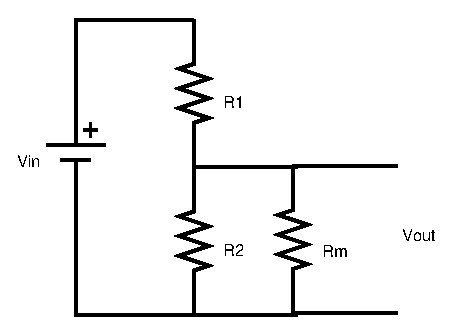
\includegraphics{Diagram2.eps}
\end{center}
%\input{Diagram2}
\caption{Resistve voltage divider with load $R_m$.}\label{fig:Resistive_VD_loaded}
\end{figure}

For $R_m = 10000\ \Omega$ and 1000 $\Omega$, $I_m = 0.00039$ A and 0.0056 A respectivly. Calculating $V_{out}$ gives
\begin{displaymath}
V_{out,\ 10000} = I_m R_m = 0.00039\ \mathrm{A}\ 10000\ \Omega = 3.9\ \mathrm{V}
\end{displaymath}
\begin{displaymath}
V_{out,\ 1000} = I_m R_m = 0.0056\ \mathrm{A}\ 1000\ \Omega = 5.6\ \mathrm{V}
\end{displaymath}
If $R_m = 0\ \Omega$, $V_{out} = 6$ V. These results demonstrate how the load on a simple voltage divider varries $V_{out}$, thus this circuit is not a good voltage source; one that provides a constant voltage independent of the load.

\subsection{Part B}
Some circuit components have a resistence that is not directly dependent on the current through them, but, rather, the applied voltage; meaning that the current is not proportional to the voltage. A light-emitting diode (LED) is an example of such a {\em non-ohmic} device. Figure \ref{fig:LED_VD} displays a circuit consisting of a resistor $R_1$ in series with a LED.
\begin{figure}
\begin{center}
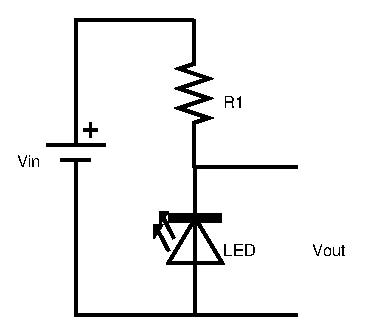
\includegraphics{Diagram3.eps}
\end{center}
%\input{Diagram3}
\caption{$R_2$ has been replaced with a LED to demonstrate the non-ohmic nature of LEDs.}\label{fig:LED_VD}
\end{figure}

The current through the circuit and voltages across the two elements were measured for each value of $R_1$ = 100 $\Omega$, 1 k$\Omega$, 10 k$\Omega$, 100 k$\Omega$, 1 M$\Omega$ while $V_{in} =5$ V. Figure \ref{fig:plot03} shows the  voltage-current dependence across the LED. For $R_1$ = 100 $\Omega$ the LED emitted bright light, 100, visable, 1000, faint, 10000 and 100000 none at all\footnote{Answer to question four.}. If the LED were an ohmic device, obeying Ohm's Law, the current-voltage relationship would be esentially linear throughout the graph because if the resistence is constant,  voltage divided by current would always have to equal the resistence\footnote{Answer to queation five.}.
\begin{figure}
\input{plot03}
\caption{Voltage across the LED versus the current across the LED showing the non-ohmic nature of LEDs.}\label{fig:plot03}
\end{figure}

\section{Discussion \& Conclusion}
For Ohmic devices the voltage across the device is directly proportional to the current running throught the device. For non-ohmic devices the voltage across and the current through the device are dependent on eachother. As demonstrated, the simple resistive voltage divider is not a good voltage source due to its dependence on the load on the circuit.

%\begin{thebibliography}{9}
% This command tells LaTeX to create "References" section containing all the references that are not commented out. Be sure to uncomment all the references which you use and add those that are not currently listed.
%\bibitem{Manual} Lab manual
%\end{thebibliography}

\end{document}
